\chapter{Network tracing}
\label{trace}

A network (or packet) {\em trace} is a record of activity of a
physical network over a period of time.  A network trace can contain
information about the length of each packet, the time it was seen and
part or all of the actual packet contents.

The emphasis of this thesis is traffic intensity with respect to time.
For this packet inter-arrival times are needed.  This is done by
recording a time-stamp in the trace.  The more accurate the time-stamp
the finer the analysis that can be performed.

For packet size analysis the length of the packet has to be recorded.
Because packet sizes are a function of higher level protocols, for any
in-depth analysis the origin of the packet has to be obtained.  This
can be done by examining the contents of each packet and extracting
the relevant information.  This is a time consuming task so it cannot
be done during the execution of the tracing program.  Instead the
first forty to fifty bytes of each packet is recorded for later
processing.

Packet traces are normally stored as large binary files.  Programs can
then examine these files and perform statistical analysis on the data.
Recording a trace over any reasonable length of time produces large
files, in the order of megabytes or tens of megabytes.

\section{Producing a packet trace}

The packet traces of Ethernet segment were collected using an IBM PC
directly connected to the Ethernet.  Because of the broadcast nature
of Ethernet it is easy to record all packets sent on the network.  The
program records a time-stamp, the packet size and the first $n$ bytes
of the packet, where $n$ is defined at compile time.

The number of packets the program records is set at compile time, and
normally ranges from ten thousand to half a million.  In a later version
of the program it should be possible to specify the number of minutes
the program is to run.

\subsection{Format of the trace file}

\begin{figure}
\begin{center}
\leavevmode
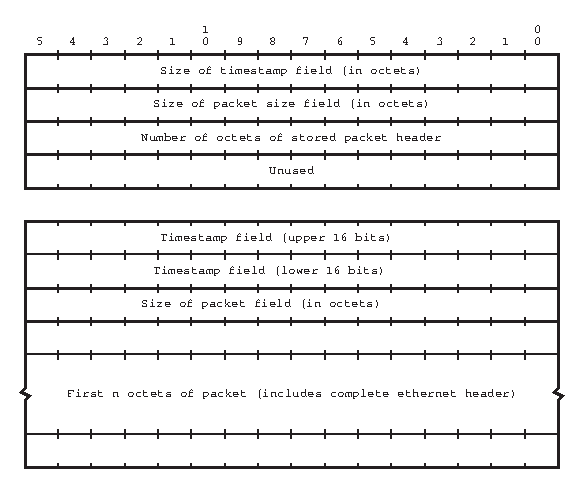
\includegraphics{pics/trace-format.eps}
\end{center}
\caption{Format of the trace file}
\label{trace:format}
\end{figure}

The trace file has an eight byte header containing four records, each
a two byte big endian word.  The contain the length of the time stamp
(in octets), the length of the packet size, the number of octets of
packet header and an unused word respectively (see
Figure~\ref{trace:format}).

Following the header are the actual trace records, which contain the
time stamp, the size of the packet (this includes the Ethernet header
but not the frame checksum) and the first $n$ octets of the
packet.

\subsection{Hardware used to produce the traces}

The hardware used was a standard IBM PC compatible with an Ethernet
controller.  This was used because it was easy to write the software
needed to produce the trace and because the hardware is widely, and
cheaply, available.  The IBM PC architecture does have several
drawbacks.

\begin{itemize}
\item	The clock used to generate the time stamps is limited in
accuracy to approximately 1 ms.

\item	The input/output bus is limited to transfers of about 700
kilobytes per second.  Very long bursts could be a problem.

\item	Interrupt events block other interrupts, causing problems
with the timer.
\end{itemize}

The Ethernet controller has an eight kilobyte buffer so as to reduce
the actual packet loses.  This may affect the analysis as queued
packets will be seen by the program as having a fixed inter arrival
time.

\subsection{Software used to generate the trace file}

The software is written in C and then compiled.  It is based on {\em
packet driver} software.  Packet drivers are pieces of code which
isolate the programmer from the specific details of each hardware
controller, presenting a standard interface regardless of the actual
controller.  This enables programmers to write much simpler programs
at the expense of a small extra overhead.

When a packet arrives at the Ethernet controller it generates a signal
to interrupt the processor and process the packet.  The packet driver,
while in interrupt mode (that is, the processor has suspended what it
was doing and is executing a special routine called an interrupt
handler) calls a user program with the size of the packet.  This
returns a pointer into memory for the contents of the packet to be
copied (this includes the packet header).  The driver copies the
packet and calls a second user program routine to tell it that the
copy has been completed.  Once the second routine has exited, the
packet driver then returns from interrupt mode, and the processor
restarts what it was originally doing.

The problem with interrupt mode is that code executing while in
interrupt mode cannot itself be interrupted (this is not strictly
correct but is true for packet drivers).  Interrupts which occur while
this happens are placed in a priority queue.  For this reason
interrupt handlers must do as little work as possible.  In general
programs just set flags and update simple data structures during
interrupt mode.

The program itself loops repeatedly checking these flags for change.
If a flag is set it then processes the packet from the head of the
data structure.  This looping is called {\em polling}.

\subsubsection{Data structures used}

The data structure consists of two fixed buffers.  While one is being
used the other is either waiting to be written out to a file or is
empty.  Each buffer has a fixed number of records into which packet
headers can be written.

The {\em Output File} is a standard C file pointer and is defined as
part of the C {\em stdio} (standard input/output) library.  This
enables the program to be portable to different operating systems.

There are also variables such as {\em Initial Time} and {\em Total
Packet Count} for determining when the program should terminate.

\subsubsection{Flow of polling loop}

\begin{figure}
\begin{center}
\leavevmode
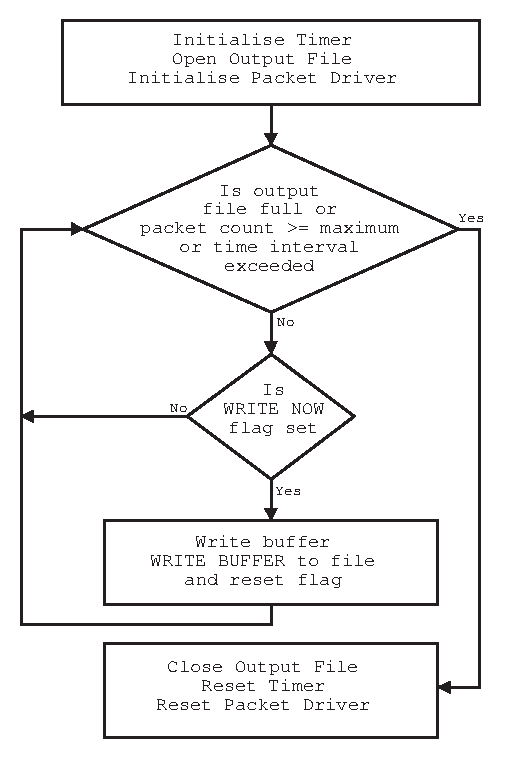
\includegraphics{pics/trace-flow.eps}
\end{center}
\caption{Flow of polling loop}
\label{trace:flow}
\end{figure}

The program has three stages.  The first initialises the required
variables and data structures, including the timer and packet driver.
The second is a repeated loop which continually checks to see if a
buffer needs to be written out to a file and the last is the final
clean up before exiting (Figure~\ref{trace:flow}).

There are various reasons for the program to terminate.  In the normal
course of events either the number of packets recorded reaches a set
amount or a running of the program exceeds a certain time limit.  Both
these values can be specified when the program is loaded into memory.
If the writing to the file should fail for some reason then the
program will also terminate.  Generally this will be because the disk
is full but other errors can occur.

\subsubsection{Flow during interrupt}

\begin{figure}
\begin{center}
\leavevmode
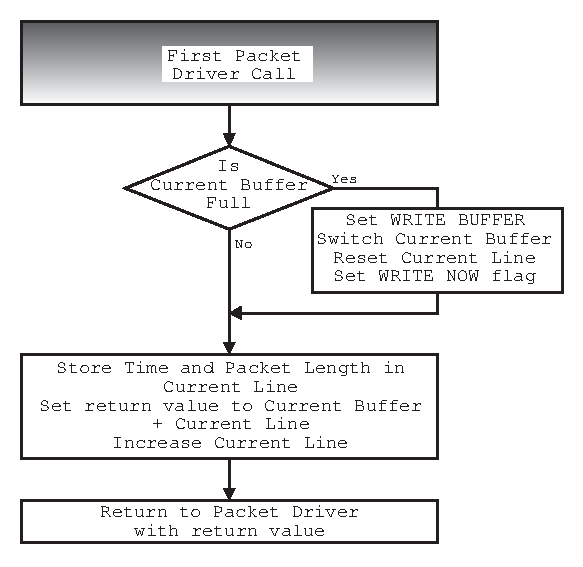
\includegraphics{pics/rcvPkt1-flow.eps}
\end{center}
\caption{Flow for first packet driver call}
\label{trace:rcvpkt1}
\end{figure}

\begin{figure}
\begin{center}
\leavevmode
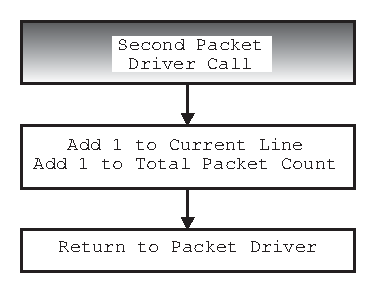
\includegraphics{pics/rcvPkt2-flow.eps}
\end{center}
\caption{Flow for second packet driver call}
\label{trace:rcvpkt2}
\end{figure}

When an interrupt is received by the packet driver it in turn calls
the user with the size of the packet and expects a pointer into memory
as a return result.  It also stores the current timer value and the
size of the packet into the current record
(Figure~\ref{trace:rcvpkt1}).

The packet driver then copies the contents of the packet into the
specified memory and calls a second user routine.  This simply updates
various counters and exits without any return value
(Figure~\ref{trace:rcvpkt2}).

\subsection{Known problems}

\subsubsection{Errors with the timer}
\label{trace:timerprob}

The timer works by having an internal 16 bit hardware counter, say
$c_0$. This starts at 0xFFFF (65535), counts down to 0x0000, then
resets itself automatically and starts counting down again.  When it
reaches 0x0002 it causes an interrupt and a counter $t$ kept by the
timer code is increased.  The counter is split into upper and lower
bytes, $c_u$ and $c_l$ respectively.  The value returned from the
timer is
\[
2^{8}t + (256 - c_u)
\]
which should theoretically always give the correct result.

The 1.19318 MHz clock generates the clock signals so that the standard
PC BIOS time is accurate to $\sim$ 18.2 Hz or 54.9 ms.  We use $c_u$
to give us a rate of 4.66 kHz or 0.2 ms.

Because the timer is asynchronous to the main processor, if $t$ should
fail to be increased at the correct time a problem may occur.  With
the Intel 80x86 processor a flag allows or blocks interrupts from
occurring.  If this flag is set then interrupts get queued, waiting
until the flag is cleared so they can occur.

If a packet arrives when $c$ is close to zero then an interrupt occurs
and the packet driver is called.  The packet driver sets the interrupt
flag (since another packet may be received while the driver is still
processing the first and if it was allowed to interrupt again the code
would probably crash).  While the driver is processing the interrupt
the timer reaches 0x0002, causes an interrupt, which is queued,
counts a little more and resets itself.

The tracing code then reads the value from the timer code, which is
now incorrect, since $t$ has not yet been incremented, and stores it
within the current buffer.  Afterwards the packet driver clears the
interrupt flags and exits, the timer interrupt occurs, $t$ is
incremented to the correct value, and the timer value is what it
should be.

The problem occurs because of a limitation of the Intel 80x86
architecture and cannot be avoided without considerable modification
of the packet driver code to stop it from having the interrupt flag
set while calling the user program code.  It is unclear whether this
is even feasible.

Because this problem is known it can be corrected in later processing
without much difficulty, so rather than try to fix it at
its origin it is simpler to make the corrections.

\subsubsection{Machine crashes after program exits}

After running the tracing program it is necessary to reboot the
machine it ran on.  This is more an inconvenience rather than a
problem.  The reason for the problem is unknown but the timer code is
the most suspect.  The amount of time needed to fix this problem is
not worthwhile and since it does not affect the results it can safely be
ignored.

\section{Testing the packet tracer}

\subsection{Introduction}

Having written this program a series of controlled experiments were
performed to check the validity and usefulness of the program.  Below
are some of the requirements of interest.

\begin{itemize}
\item	At what rate of packet arrival does packet loss occur?

\item	Does the size of the arriving packets affect packet loss?

\item	In what form does packet loss happen?

\item	How is packet loss affected by writing to permanent storage?
\end{itemize}

\subsection{Design}

This experiment was performed using two machines connected via an
isolated segment of Ethernet.  On one machine a packet generator
executes while the other records all packets seen on the segment and
writes them out to permanent storage.

One important note is the relative processing power of each machine.
While both machines have compatible architectures one is at least
twice as fast as the other.  This asymmetry enables the recording
program to be ``tested to destruction'' while the packet generating
machine remains stable.

The experiment was carried out by subjecting the recording machine to
various traffic loads (as specified by the generator's input
parameters) and examining the resulting output file.

\subsection{The packet generator}

The packet generator generates $c$ packets of fixed size $s$ octets.
Between the start of each packet is a delay $d$ ticks where a tick is
$\sim$ 0.2 ms.  If the time required to send a packet is greater than
the specified delay then the packets are sent end to end without any
artificial delay.  These three parameters can be specified on the
command line.

{\small
\begin{verbatim}
stress [-s packet size] [-c number of packets sent] [-c delay]
\end{verbatim}
}

$stress$ uses packet drivers for it communication with the Ethernet
hardware.  The code consists of a single loop which continually sends
out packets using the Ethernet broadcast address.  The current
sequence number and time follow the address within the packet.


\subsection{Experiment - determining the maximum output rate}

\begin{figure}
\leavevmode
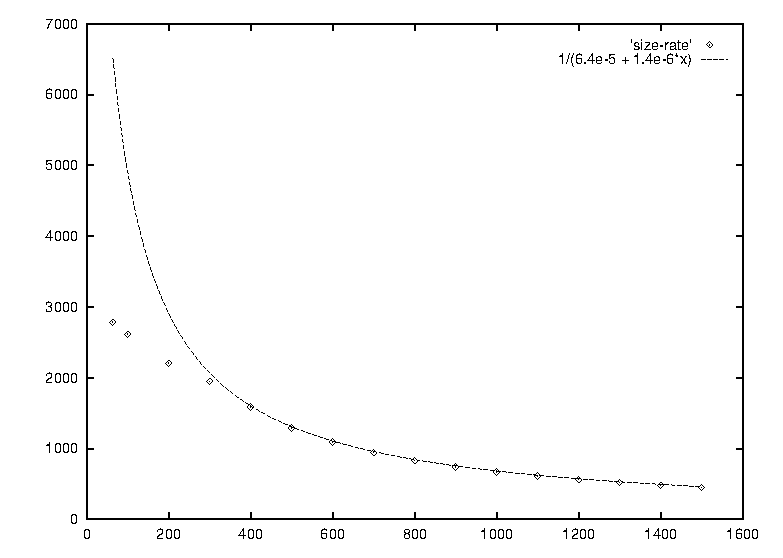
\includegraphics{pics/size-rate-fit.eps}
\caption{Output Rate versus Packet Size}
\label{trace:expr1}
\end{figure}

\begin{figure}
\leavevmode
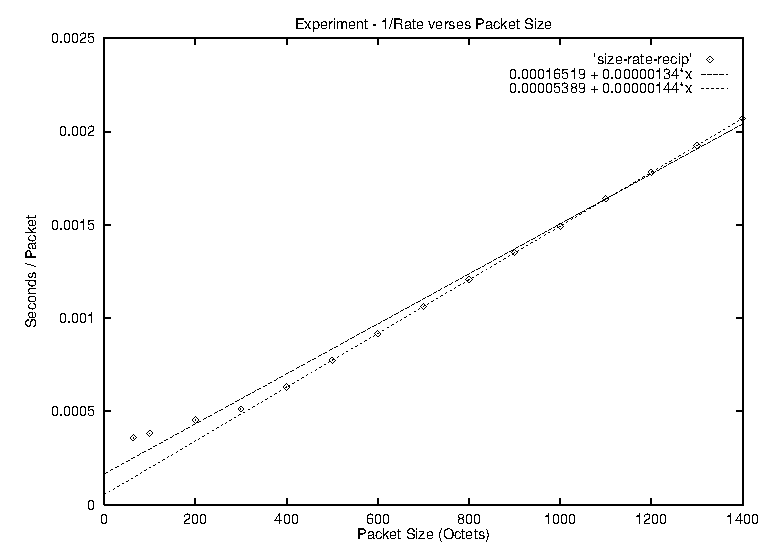
\includegraphics{pics/size-rate-recip.eps}
\caption{1 / Rate versus Packet Size}
\label{trace:expr3}
\end{figure}

\begin{table}
\begin{center}
\begin{tabular}{ccc}
{\bfseries Packet Size} & {\bfseries Packets per} & {\bfseries Octets per} \\
{\bfseries (octets)} & {\bfseries second} & {\bfseries second} \\
0064	& 2785 & 178240 \\
0100	& 2616 & 261600 \\
0200	& 2206 & 441200 \\
0300	& 1948 & 584400 \\
0400	& 1586 & 634400 \\
0500	& 1290 & 645000 \\
0600	& 1090 & 654000 \\
0700	& 0941 & 658700 \\
0800	& 0828 & 662400 \\
0900	& 0740 & 666000 \\
1000	& 0670 & 670000 \\
1100	& 0610 & 671000 \\
1200	& 0561 & 673200 \\
1300	& 0519 & 674700 \\
1400	& 0483 & 676200 \\
1500	& 0451 & 676500 \\
\end{tabular}
\end{center}
\caption{Results for maximum rate experiment}
\label{trace:expr2}
\end{table}

To examine the behaviour of the packet generator a series of packet
generations was carried out from the slower to the faster machine.
The experiment looked at the maximum rate (in packets per second) the
generator could produce given a specific packet size.  The result can
be seen in figures \ref{trace:expr1} and \ref{trace:expr3}, and
table~\ref{trace:expr2}.

These were produced by sending 10,000 packets back to back without
delay between the two machines.  The trace file is then analysed and
the number of packets per second is extracted using {\ttfamily arrival}.

The curve on figure \ref{trace:expr1} was produced by taking the
resulting values (table~\ref{trace:expr2}, ignoring the first four
values, taking the reciprocal and fitting a linear line to it.  In
figure~\ref{trace:expr3} you can see both line fits, one including all
the points and the other excluding the first four points.  This linear
fit was then inverted and plotted against the original points.

The results suggest that beyond packet sizes of 400 octets the
generator's output is bounded by the I/O (Input / Output) of the
machine, at about 710,000 octets/second or 693 K per second.  Packet
sizes smaller than this are bounded by the processing time needed to
send each packet so that the curve represents the maximum theoretical
output in packets per second.

Note that 710,000 octets/second is less than Ethernet's theoretical
throughput of around 1,200,000 octets/second so that on a faster
machine with greater I/O bandwidth more than 700 K per second is
easily achievable.

\subsection{Summary of packet trace test}

\begin{itemize}

\item
No losses were observed in the experiment, and th packet rates used
there are higher than those observed on the Campus network.

\item
In the experiment there was on evidence of packet loss during writes
of the trace data to disk storage.

\end{itemize}

Overall the trace program performed very well, providing a simple and
effective tool for collecting network traffic data.
